\chapter{INTRODUCTION}
\label{ch:intro}

\textbf{Motivation---why you should read this thesis
What is this thesis about?}
% At first glance, the Universe appears to be an overwhelmingly vast and complicated place.
% However upon closer inspection, it is comprised of only a few different kinds of fundamental particles.
% Particle physics has given rise to the Standard Model (SM) which mathematically describes these constituents and their interactions with each other.
The universe, while overwhelmingly vast, is comprised of a curiously small number of unique elementary particles.
These particles---and their interactions with each other---are accurately described by the standard model (SM) of particle physics.
% strong, weak, and electromagnetic interactions

% By understanding the rules by which these particles interact, we can ;
% this is the aim of the Standard Model (SM) of Particle Physics. 
% The Standard Model (SM) is an impressively accurate mathematical theory which describes the fundamental particles of the universe and the rules for their possible interactions.
% Problematically though, the SM predicts that all particles are massless.
%  are described mathematically by the impressively accurate Standard Model (SM) of Particle Physics.
% Although there are four fundamental forces of nature, the SM takes into account three of the four forces in nature:
A major shortcoming of the SM was its inability to predict the masses of these particles.

The SM was not able to predict the masses of these particles until 1964 when the Brout-Englert-Higgs mechanism suggested that 
It wasn't until 1964 that the Brout-Englert-Higgs mechanism gave a self-consistent way to :
by breaking the electroweak gauge symmetry of the vacuum would give rise to non-zero masses of the weak gauge bosons.
This would yield a secondary effect too:
there should exist a fundamental scalar boson which is the quantum of the so-called ``Higgs field''.
On July 4th, 2012, this Higgs boson was discovered.

This dissertation presents the world's most precise measurement of the Higgs boson mass (\mH) to date, using proton-proton collision data from the LHC Run 2, collected and analyzed by the CMS Experiment.
The value of \mh has been measured previously TODO:CITE LOTS OF PEEPS~\cite{hig16041} but it is important to always strive for lower uncertainties (\ie to increase the precision) on the mass value, since the very stability of our universe is theoretically dependent on it, as shown in Fig.~\ref{fig:universe_stability}.
% Additionally, the value of \mh is one of the free parameters of the SM and is theoretically linked to the very stability of our universe.
Furthermore, the value of \mh sets limits on the masses of the other particles.
% Universe metastability.
%%%%%%%%%%%%%%%%%%%%
\begin{figure}[hbtp]
    \centering
    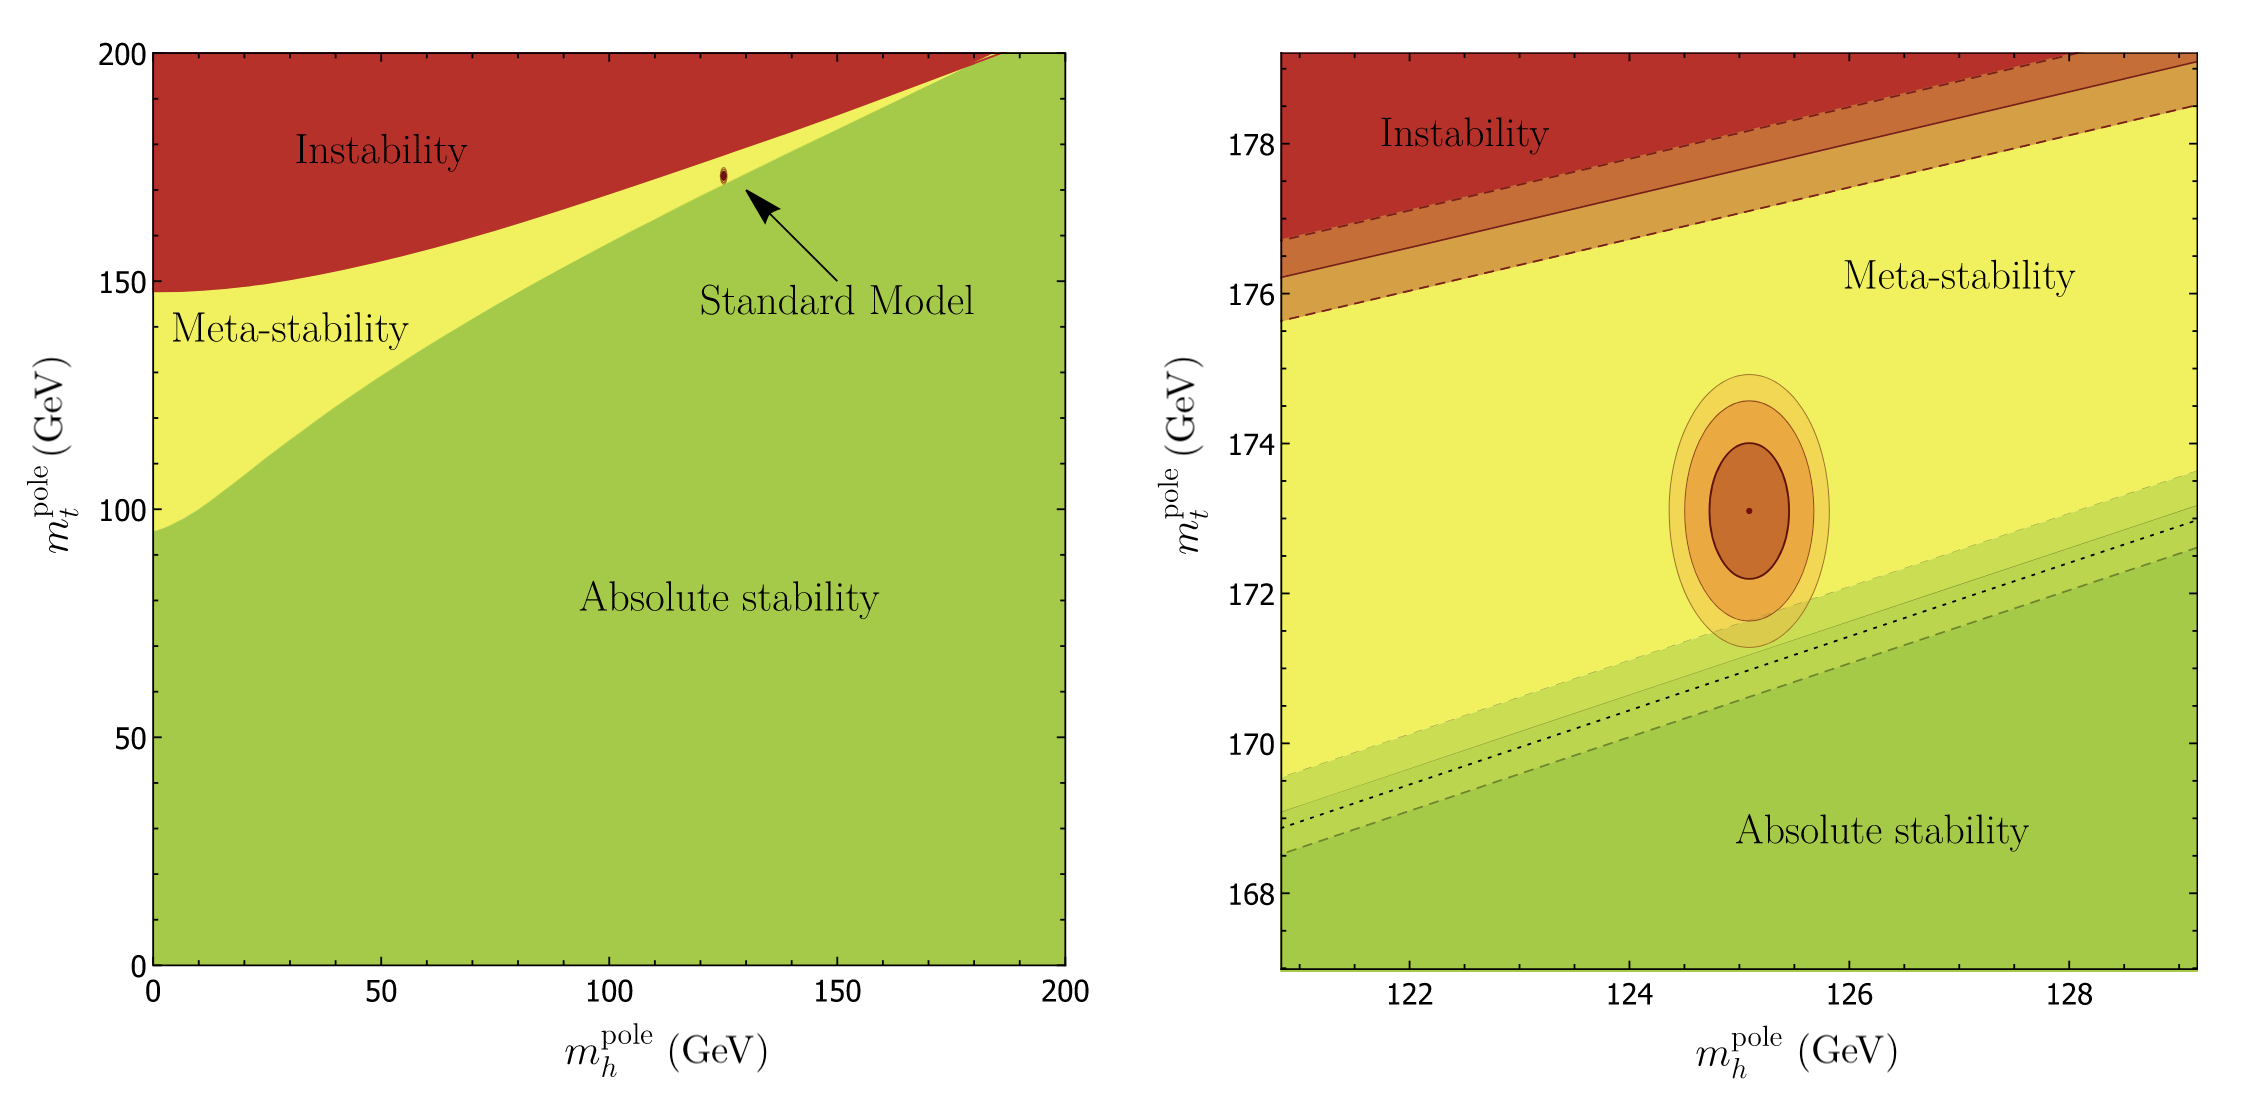
\includegraphics[width=15cm,height=10cm,keepaspectratio]{figures/intro/mtop_vs_mH_universestability.png}
        \caption{
        (Left) Theoretical stability regions of our universe based on the pole masses of the top quark $\left( \mass{t}^\text{pole} \right)$ and Higgs boson $\left( \mass{h}^\text{pole} \right)$.
        (Right) A closeup of the SM region of the left plot.
        The contours represent the 68\%, 95\%, and 99\% confidence levels based on the experimental uncertainties of $\mass{t}^\text{pole}$ and $\mass{h}^\text{pole}$.
        Plots taken from~\cite{univ_stab} and units added to all axes.
        }
        \label{fig:universe_stability}
\end{figure}
%%%%%%%%%%%%%%%%%%%%

The measurement of \mH presented in this dissertation utilizes the following improvements compared to previous measurements:
\begin{itemize}
    % More data.
    \item more analyzed data (TODO:LATEXCOMMAND cf. $\lumi(2016) = \lumisixteen$ \vs $\lumi(\text{Run2}) = \lumiruntwo$)
    % Four final states (instead of three).
    \item Four final-state categories are used: \fourmu, \foure, \twoetwomu, \twomutwoe.
    In previous measurements, the last two final states (the mixed-flavor states) were combined, but they have different kinematical properties, depending on into which lepton pair the \Zone decayed:
    they have different peak widths (instrumental resolutions), different signal efficiencies, and different relative levels of reducible background.
    % Using UL reco (better electron pT resolution).
    \item Ultra-Legacy (UL) reconstruction is used for muon, electron, photon, and jet tracks.
    This signficantly improves electron momenta, while improving the other particle momenta a little less so.
    % Vertex constraint.
    \item The measurements of muon \pt are improved by constraining the muon tracks to originate from the interaction vertex (also called a \emph{vertex constraint}).
    \item TODO:REWORD A correlation between \mfourlerr and \Dkinbkg is avoided by 
    When extracting the value of \mH in past measurements, a 3D $\text{pdf} \left( \mfourl, \Dkinbkg, \mfourlerr \right)$ was built into a factorized form
    $f \left( \mfourl, \mfourlerr \middlepipe \mH \right)   \cdot   g\left( \Dkinbkg \middlepipe \mfourl \right)$,
    which was later found to contain an existing correlation between \Dkinbkg and \mfourlerr.
    To account for this correlation, now the events are split into 9 categories based on the per-event \emph{relative} mass uncertainty $\left( \relmfourlerr \right)$ and, for each, a 2D $\text{pdf} \left( \mfourl, \Dkinbkg \middlepipe \mh \right)$ is built.
    % Z1 mass constraint.
    % \item Just as was done in the 2016 \mH measurement~\cite{}TODO:CITE, a \Zone mass constraint is imposed on events with the \fourmu and \twomutwoe final states to improve the momenta of the two muons comprising the \Zone.
    % The improvement here is that now the muon tracks are constrained to come from the interaction vertex in the fit (sometimes called a \emph{vertex constraint}).
    \item The uncertainties on lepton momentum scale ($\pt^{\Pe, \mu}$) are reduced, thanks to a more detailed analysis of the corresponding systematic uncertainties.
    This has the additional effect of significantly reducing the uncertainty on the per-event four-lepton mass resolution.
\end{itemize}

This dissertation is organized into the following chapters:
Chapter~\ref{ch:intro} (\emph{this chapter}) discusses the importance and motivation for measuring the mass of the Higgs boson;
Chapter~\ref{ch:theory} introduces the standard model (SM) of particle physics and its mathematical framework, including the Brout-Englert-Higgs (BEH) mechanism;
Chapter~\ref{ch:lhc};
Chapter~\ref{ch:cms};
Chapter~\ref{ch:higgs_mass};
Chapter~\ref{ch:dilep_res};
Finally, Chapter~\ref{ch:conclusion}.
